\mode*
\part{Getting Started}
\lecture{intro}{intro}% \lecture[short name]{name}{label}

\begin{frame}{Linux Commands}
  \begin{description}
  \item[Where to find them?] {\ttfamily /bin, /usr/bin, /usr/local/bin,\\\symbol{`~}/bin,
      \ldots}
    \begin{itemize}
    \item[\$] \texttt{echo \$PATH}
    \end{itemize}
  \item[How to find them?] \texttt{which, whereis, type}
  \end{description}
  \begin{block}{Command not found?}
    \begin{description}
    \item[First] double check your spelling
    \item[Then] try:{\ttfamily
      \begin{itemize}
      \item[\debian] aptitude search xxx
      \item[\debian] apt-cache search xxx
      \item[\debian] apt-file search xxx
      \item[\debian] sudo apt install packagename
      \item[\GG] \google~"linux command xxx"
      \end{itemize}}
    \end{description}
  \end{block}
\end{frame}

\begin{frame}{Text Editors}
  \begin{iblock}
    {\mode<beamer>{{{\Huge\vim}\,\quad{}vs.\quad{}{\LARGE\emacs}}}
      \mode<article>{{\vim\,\quad{}vs.\quad{}\emacs}}}
    \begin{center}
      \mode<beamer>{ 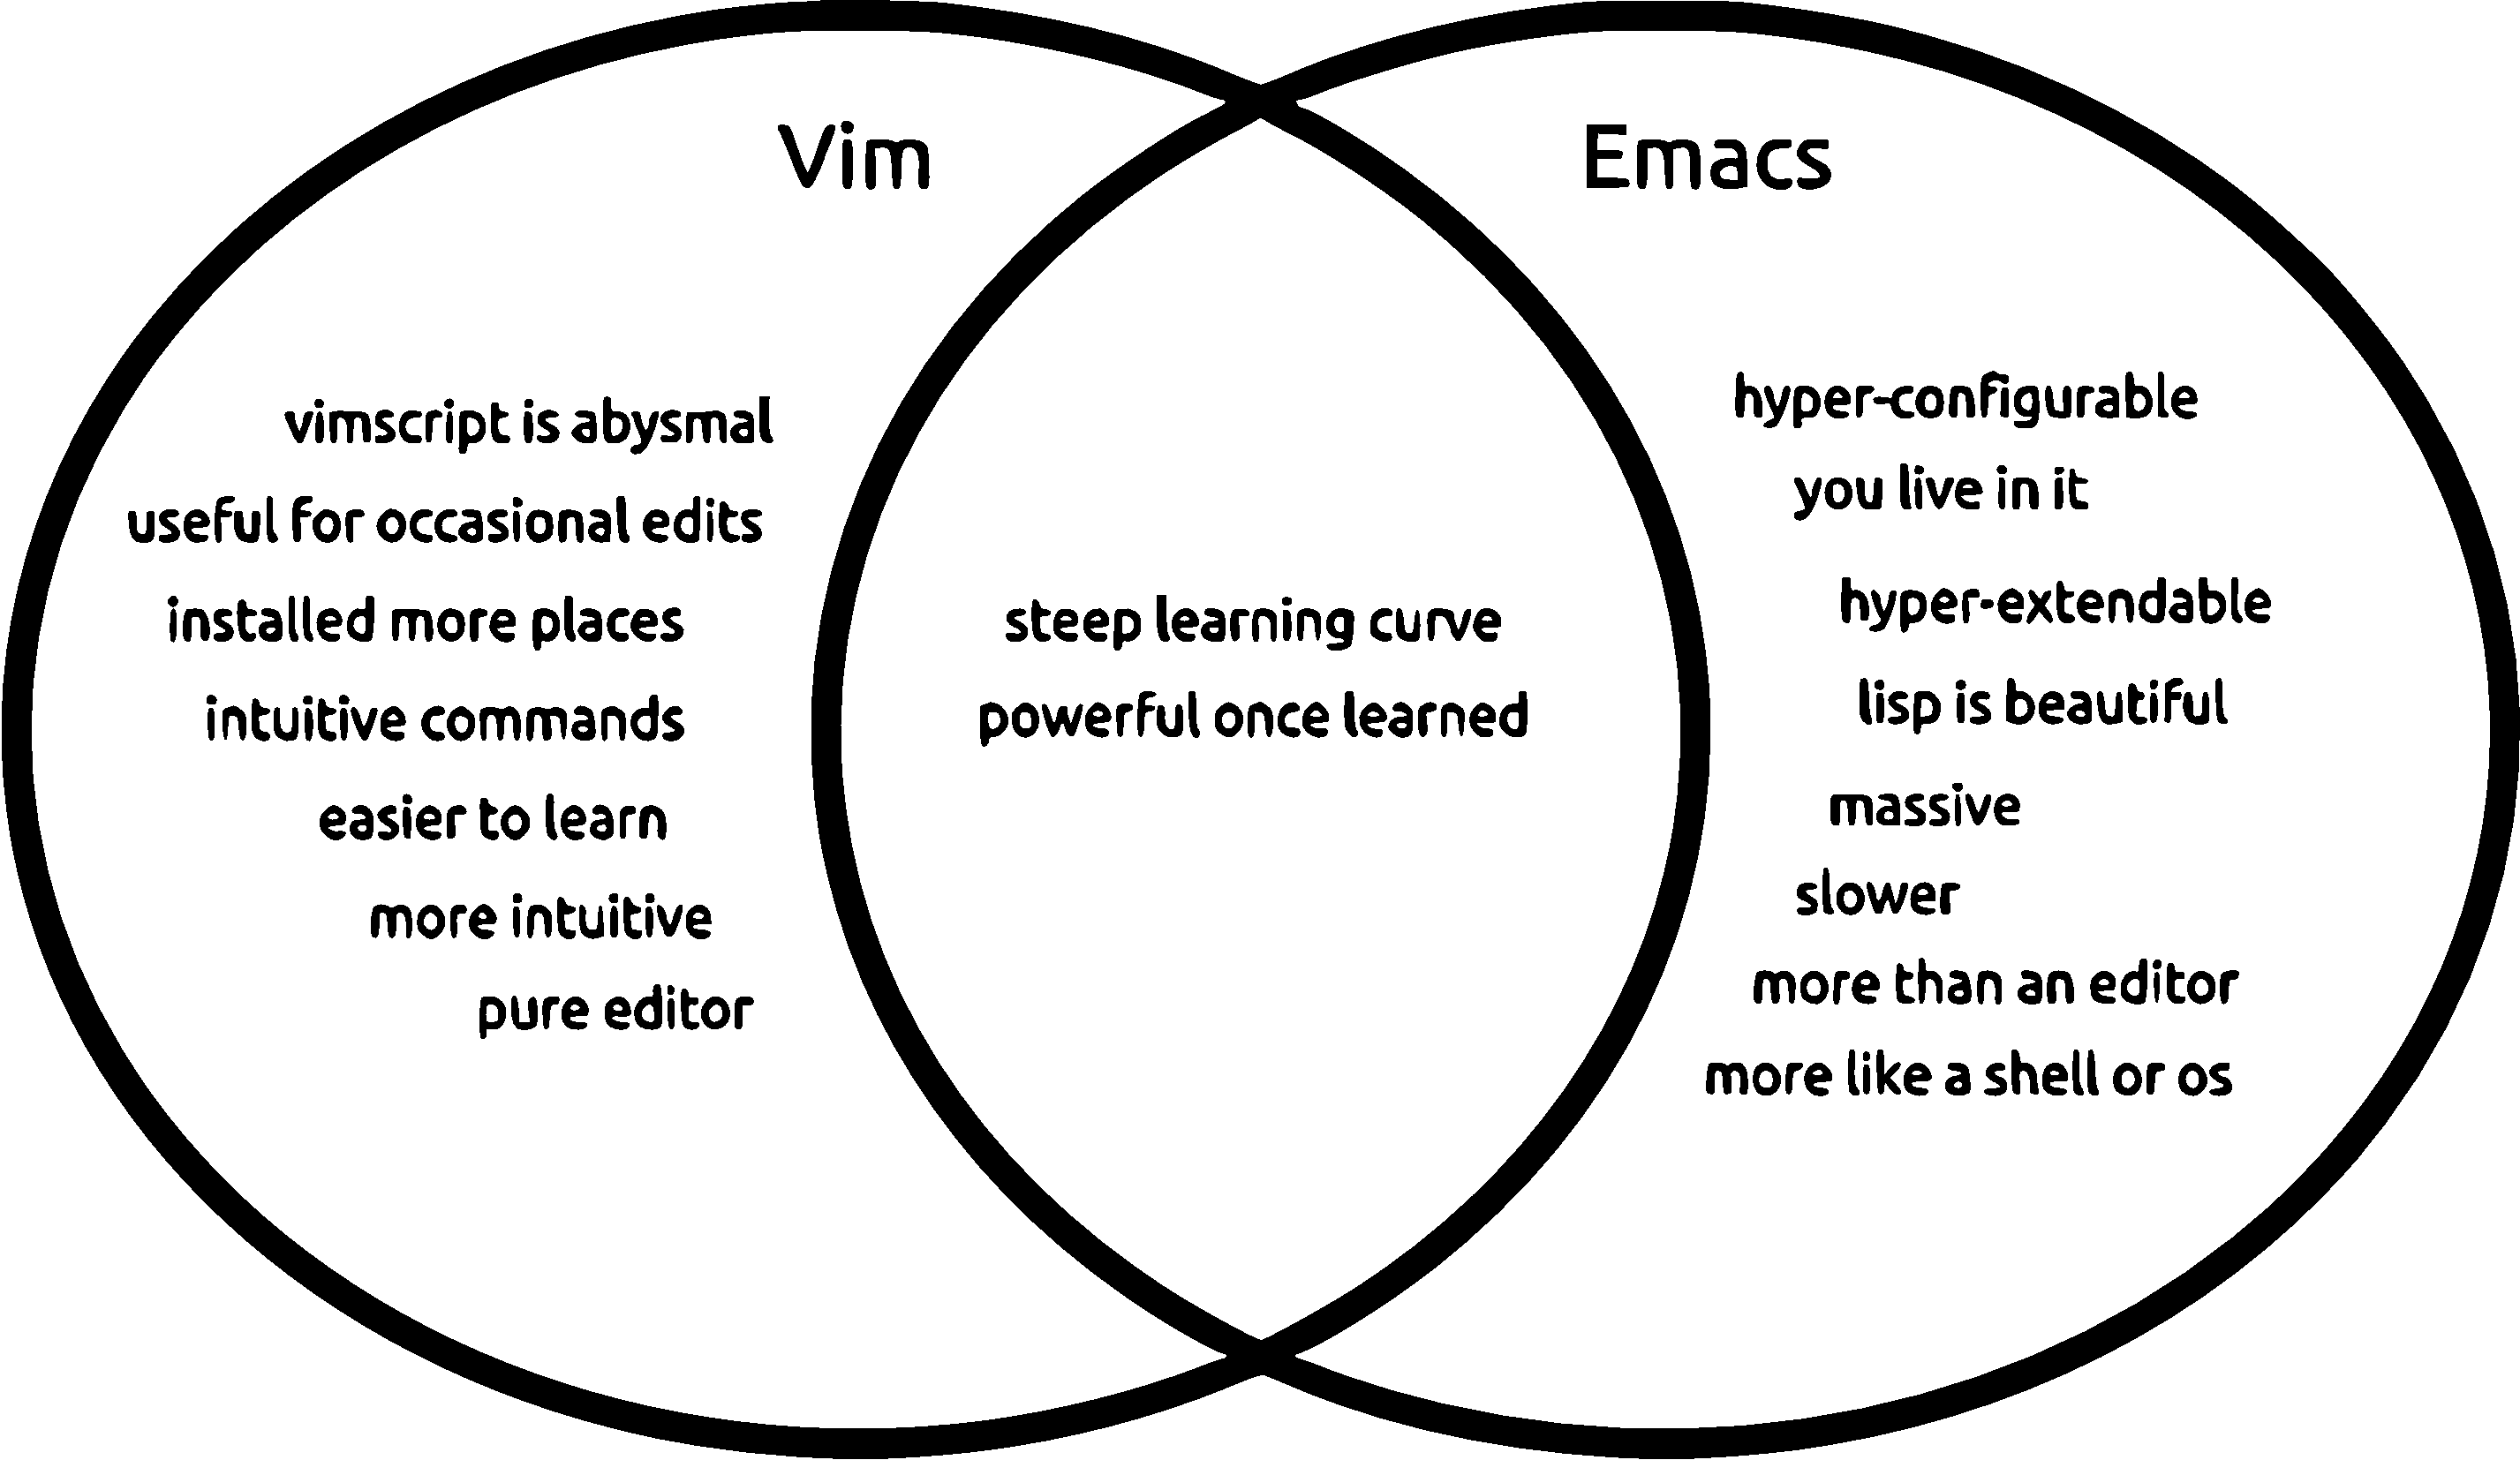
\includegraphics[width=.7\textwidth]{vivsemacs} }%
      \mode<article>{ 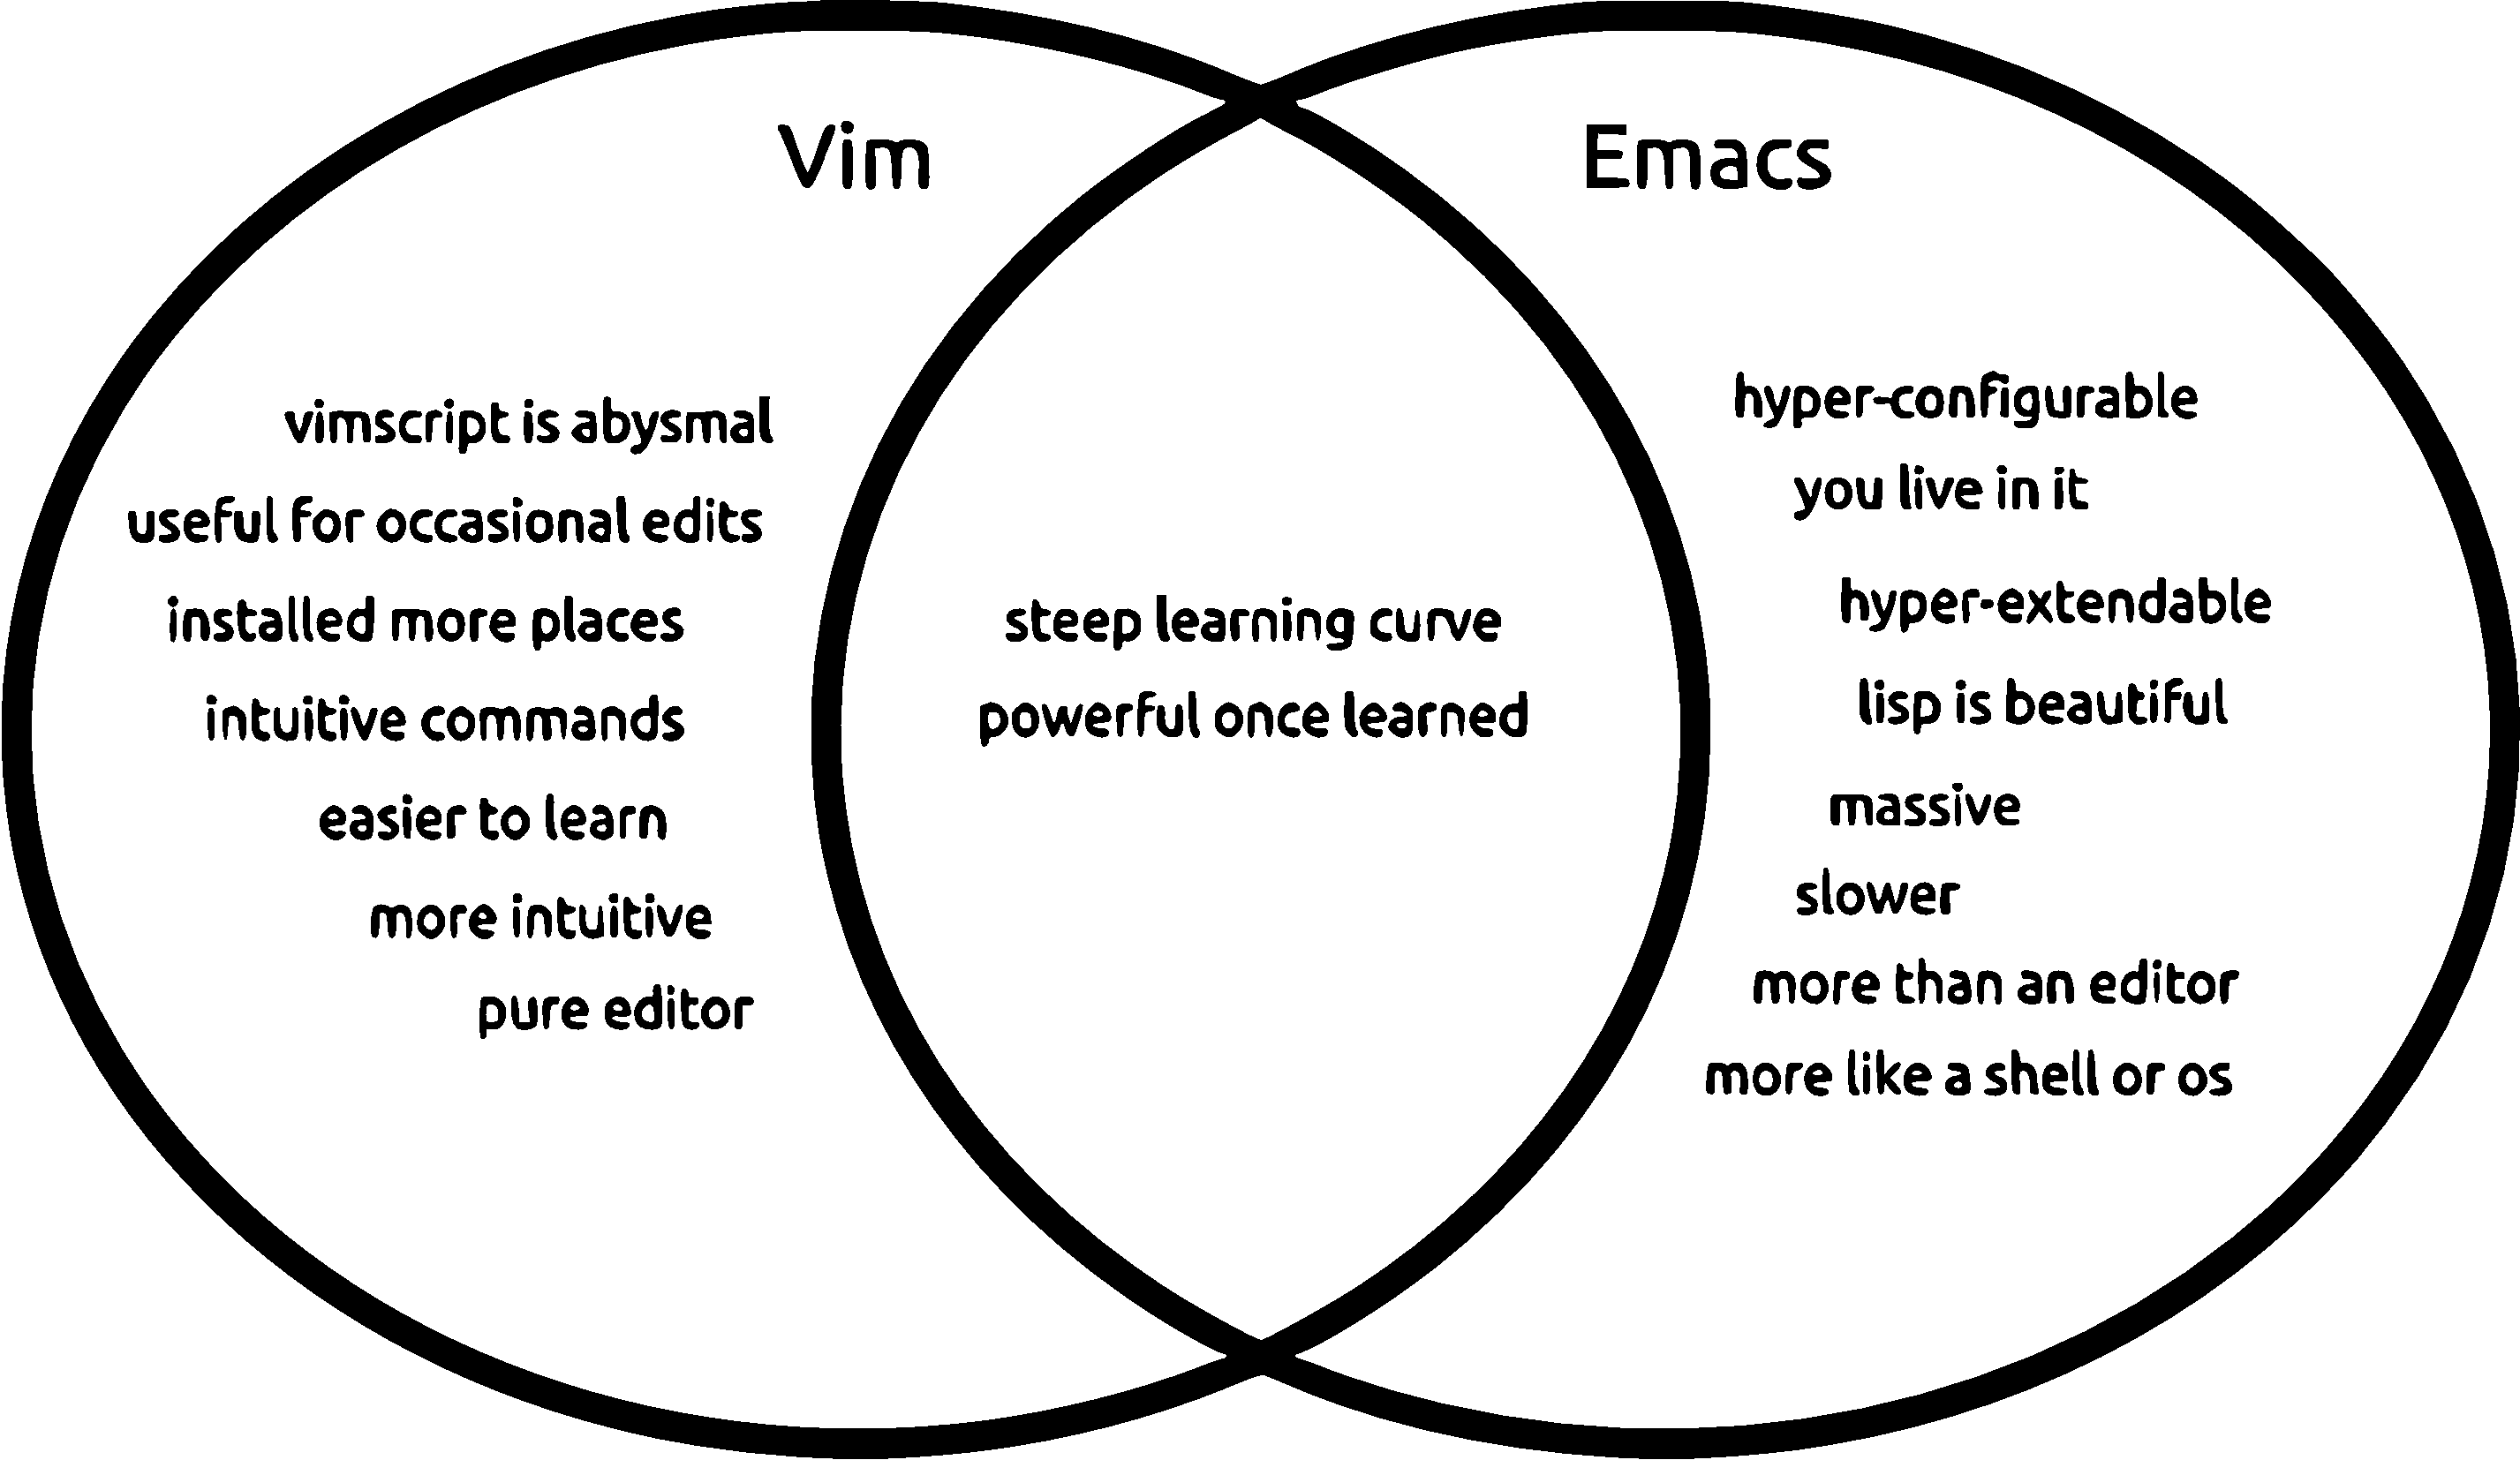
\includegraphics[width=.5\textwidth]{vivsemacs} }
    \end{center}
  \end{iblock}
  \begin{description}
  \item[uemacs] Linus Torvalds' editor
    \begin{itemize}
    \item[\github] \url{https://github.com/torvalds/uemacs}
    \end{itemize}
  \end{description}
\end{frame}

\begin{frame}{Help Your Editor}
  \begin{iblock}{Suffix matters}\ttfamily
    \begin{itemize}
    \item[\$] vim \wrong
    \item[\$] vim hello \wrong
    \item[\$] vim hello.c  \correct
    \item[\$] vim hello.py \correct
    \item[\$] emacs \wrong
    \item[\$] emacs hello \wrong
    \item[\$] emacsclient hello.c  \correct
    \item[\$] emacsclient hello.py \correct
    \end{itemize}
  \end{iblock}
\end{frame}

\begin{frame}{Keyboard}
  \begin{center}
    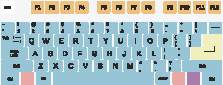
\includegraphics[width=.7\linewidth]{qwerty}
  \end{center}
  \begin{itemize}
  \item[\vim] vimtutor
  \item[\emacs] \Ch{} {\kbd t}
  \end{itemize}
\end{frame}



\mode<all>
%%% Local Variables:
%%% mode: latex
%%% TeX-master: "lap-b"
%%% End:
